\message{ !name(chap-domino.tex)}
\message{ !name(chap-domino.tex) !offset(-2) }
\chapter{Domino计算模型}
\label{chapter:domino}
随着大数据时代的到来,人们每天能够搜集和存储的数据越来越多,并且这些数据中富含了各种有用的信息。比如很多电子商务网站会记录用户的浏览历史,甚至是用户在网站中浏览时鼠标停留的位置和时间。对每一个用户来说,这些记录的数据量并不大,但是对于通常能够拥有上亿用户的电子商务网站来说,记录这些数据就需要足够的资金来建立海量存储系统。然而公司愿意付出成本来记录这些信息,并不是单纯的为了应用'海量'存储系统,而是因为这些数据确实能为公司带来利润。事实上通过对用户行为的分析,公司能够非常准确的识别出每一个用户的特征、喜好、需求,并且针对性的给予推荐商品,从而极大的提高广告到实际购买的转化率。因此存储和处理这些数据也成为了此类公司的核心技术。除了存储处理这些本身就在赛博空间(Cyber Space)存在的数据之外,越来越多的物理世界数据开始被数字化并且搜集以加以利用。比如实时交通路况数据,街景信息,停车位信息,甚至是热门饭店的排位信息都在不断的产生,转化,存储。在这些数据被存储之后,更重要的就是如何处理以利用他们。我们在第二章介绍了在云环境下现有的计算框架和模型以及他们的优缺点,在这些工作的基础上,本章将介绍一种基于触发器的新型云计算平台中的计算模型——Domino。该计算模型包括了编程模型、运行时支持、以及容错、调度、检测等部件,并且通过与现有的云计算存储系统以及前章所讲Sedna存储系统的整合,为开发人员提供了一个简单、直观、高效的大规模应用开发环境。Domino通过整合HBase存储系统来为应用开发人员提供了完整的存储和处理基础设施来更加容易的编写那些包含了大规模的迭代和递增处理的应用程序。我们基于Domino模型也实现了一系列的类似的应用,比如PageRank排序、一些比较典型的机器学习和数据挖掘算法($K$-means, 协同过滤等)、分布式的爬虫等。通过这些应用的编写和性能对比试验,我们认为Domino具备了比现有的云计算模型更加灵活的特点,并且相比较传统的MapReduce以及其扩展模型,更是具备了更好的效率和简洁的编程接口,更重要的是,Domino还为我们的大规模分布式应用程序提供了实时的容错恢复能力,这一点是现有的模型很难做到的。

那么本章将通过一下几个方面来具体的介绍Domino编程模型以及其实现:在\ref{section:intro}中,我们将综合PageRank的例子来介绍什么叫做“基于触发器的”编程模型以及为什么使用触发器模型来进行编程;在\ref{section:sync}中,我们将着重介绍Domino中的同步模型;\ref{section:design}具体的介绍Domino的实际设计与实现的细节;\ref{section:apps}将会就几个典型的应用介绍如何在Domino中实现进行详尽的介绍;最后,通过在\ref{section:exp}中通过一系列的试验检测Domino本身的性能以及其上运行的应用程序的性能。

\section{模型介绍}
\label{section:intro}
大量像Amazon EC2或者Windows Azure等IaaS基础设施服务的出现使得按需获取大规模计算资源成为可能,也极大的促进了大规模应用的出现。然而,正如过去几十年计算机的发展所揭示的那样,设计和实现不同种类的可扩放的应用程序依旧非常困难,特别是对于需要大规模计算的领域专家而言,他们除了需要考虑应用本身的分布式实现之外,还需要考虑竞争条件、死锁、分布式状态管理、同步等非常复杂的技术问题。为了把应用开发人员和这些繁琐复杂的分布式问题分隔开来,大量的分布式编程模型开始大量的出现。

这些编程模型中很大一部分是同步的数据流模型,这些模型针对的是那些面向数据流,并且对数据流进行同步的多轮处理的应用程序。比较典型的代表如MapReduce以及Dryad模型,以及一些基于它们的扩展模型。这些模型非常适合处理那些不需要访问全局共享状态的批处理应用,像\textit{wordcount}或者\textit{sorting}能够被很容易的在该模型下实现,然而很多递增或者迭代的应用就不是很适合。还有一些编程模型提供了一个面向数据的编程模型,比如Piccolo以及Pregel,这些模型提供面向对象的数据访问语义,允许用户直接访问任意的数据而不须将数据抽象为数据流来处理。由于没有数据流的概念,该类模型需要引入全局屏障(global barrier)以同步程序的执行。于此对应的是很多提供了异步语义的面向数据的编程模型,比如Oolong以及GraphLab等,其中GraphLab是一个针对图应用设计的编程模型,用户需要将其需要解决的问题抽象成为图算法来解决,这在某种程度上也限制了其应用范围。Oolong和Percolator属于另一类编程模型,它们针对递增处理应用而设计,其中Percolator使用分布式事务来管理程序执行的状态,Oolong则是通过用户提交的聚合函数作为全局屏障来同步程序的执行。然而这类面向递增处理应用而设计的编程模型太过简单,并且非常有针对性,无法作为一种通用的编程模型出现。

面对这些编程模型的问题,我们提出了一种基于触发器的通用编程模型,称为Domino,它特别适用与高性能的迭代和递增程序中,并且作为一种通用模型可以用于类型广泛的各种应用中。Domino的应用是通过组合一系列的触发器实现的,这些触发器是由用户编写的代码块组成,并且在特定的事件发生的时候被触发执行,同步或者异步程序都可以很容易的在Domino中加以实现。Domino同时提供了一个面向数据的语义。我们认为Domino具备一下几点创新性:

\begin{itemize}
\item Domino是一种通用的基于触发器的编程模型,它同时支持同步或者异步的应用程序。
\item Domino作为一种触发器的编程模型为用户提供了实时的容错恢复的能力,并且通过一系列的优化为高性能应用提供性能支持。
\item Domino和其他编程模型之间的合作能够进一步完善云计算基础软件架构。
\end{itemize}

\subsection{触发器模型}
触发器的概念在计算机科学中出现已经超过30年了。很多传统系统中,组件需要对刚刚更新的对象进行识别并且针对性的执行一系列的操作。普遍认为这种方式能够提供更好的软件模块化能力,因为更新模块和处理该更新的模块可以独立起来。比如,一个雷达物体扫描程序会不断的更新敌军飞行器的位置,那么我们系统中应该同时有一个基于敌机出现或者位置改变发射火箭进行摧毁的模块来响应雷达扫描程序的输出。通常有两种做法来完成此类工作:一种是该模块不断的检查(“轮询“)感兴趣的对象,并且当发现对象发生改变时执行特定的动作。此方案最大的缺陷就是浪费资源,并且响应时间完全受限与轮询的时间间隔,而若设置较小的时间间隔,会浪费更多的资源。另外一种则是模块在某处等待直到感兴趣的对象发生改变才被激活执行特定的动作,我们也称之为触发模型或者在某些上下文语境下也成为异步模型。

从上个世纪90年代起,数据库领域就出现了一波研究主动数据库(Active database)的热潮,核心概念就是提出一种面向数据库的主动执行的概念来简化编写数据库上应用。在主动数据库中,数据库操作或者外部的事件在满足一定条件的基础之下都能够触发特定动作执行。从概念上来说,主动数据库中的执行流程满足ECA规则,ECA即Event-Condition-Action。当一个事件发生的时候(On Event),并且特定的条件被满足了(IF CONDITION),然而指定的动作就将被执行(THEN ACTION)。主动数据库后来被广泛实现于商用数据库系统中(一般都是通过触发器或者触发器过程来实现),比如Postgres,HiPAC,Sybase,VBase以及OOPS等。然而直到今天,我们可以发现,虽然在理论上已经有很多关于ECA规则的研究,然而在主动数据库中,触发器依然是作为一个保持数据一致性、完整性或者安全检查的辅助工具存在于数据库中,一直没有成为比较通用的编程模型,其中主要原因是其复杂度太高。虽然相比较传统的面向程序的编程模型,基于触发器的编程模型能够在触发器数目较小的情况下提供明显的响应速度提升,并且通过将较大的应用分解成为一个个小的触发器来模块化应用并加以管理,不过,由于触发器对数据库领域最为核心的ACID特性,特别是事务机制的挑战,使得其一直没有成长为一个通用的模型。

不过情况在分布式环境下开始发生变化。根据之前介绍的CAP所描述,在一个分布式的系统无法同时提供一致性、可用性以及分割容忍三个特性。而且现有的云环境中,我们更加重视可用性和分割容忍性,因此一致性往往成为我们牺牲的唯一选择。在新的NoSQL或者NewSQL的分布式存储系统中,我们基本上放弃了ACID的特性,转而尝试提供最终一致或者单节点内的原子性等。在这种情况下,触发器模型也逐渐成为一个好的选择。

\subsection{Domino的编程模型}
Domino严格遵守了触发器模型,它将一个用户程序抽象为:事件监控、条件判断、以及动作执行三个部分。为了更清楚的展示如何使用Domino模型来编写应用程序的,我们这里使用一个简单的分布式爬虫作为例子来介绍。

\begin{Sbox}
\begin{minipage}{5in}
\setlength\parindent{1pc}
\textbf{[分布式爬虫实例]}最基本的分布式网页爬虫非常简单,它开始于几个简单的网页URL地址,爬虫会不断的将这些网页读取下来并且进行分析,通过分析网页的外链,爬虫将会获得更多的网页URL地址,周而复始直到爬取到某种限额或者整个网络。当然,一个可以工作的网络爬虫不止这么简单,它需要遵守Robots协议,需要考虑到网络带宽,需要考虑页面更新等等。而在我们的这个简单的例子中,我们并不会把重心放在这些功能上,而是更加关注网络爬虫的核心功能:爬取页面,分析页面。

我们的爬虫并不是爬取互联网上的网站数据,而是爬取一个新型的社交网络上的信息(新浪微博)。微博是一种新型的社交媒体,所有的用户都可以发表公开的不超过140字的消息或者评论、转发他人的消息。由于其简单且交互性强而越来越活跃。我们不希望爬取所有的微博上的信息,而是希望能够爬取最新的消息,并且希望我们的爬虫可以以更高的优先级爬取那些更重要的消息。这里的更重要使用了一个评论数加转发数的方式来定义,如果一个消息的评论数和转发数更多,那么它就更加重要。

基于Domino实现的网络爬虫程序总体结构如下:需要两个触发器的相互配合,触发器\textit{WBContentTrigger}负责监控微博消息表,当其中出现新的微博的时候,需要该触发器获取该微博的所有评论或者转发的用户的信息,并且写入到微博用户信息表中;而触发器\text{WBUserTrigger}负责监控微博用户信息表,当该表中某一个用户状态发生改变,意味着最近该用户曾经评论或者转发过别的用户信心的时候,该触发器将负责爬取这个用户最近的微博消息,并且写入到微博消息表中。
\end{minipage}
\end{Sbox}
\shadowbox{\TheSbox}

\subsubsection{事件(Event)}
那么触发器模型中,首要的元素就是ECA中的Event即事件。事件的种类非常多,按照之前在主动数据库中的分类,事件一般可以被划分为简单事件和复杂事件。其中简单事件主要包括了:时间事件(包括绝对时间事件和相对时间事件),方法事件(比如某个方法被调用而产生的事件),事务事件(比如事务提交或者准备事件),以及数据事件(比如数据被读取或者写入产生的事件)等。而复杂事件则是简单事件的组合或者是使用简单事件加上某些特定语义来组合,比如在某一个时间周期内未出现某个事件就被认为是一个复杂事件等等。然而在Domino中,我们主要关注的应用场景就是希望对存储在系统中的数据变化进行监控,因此我们主要提供了数据事件,特别是写数据事件的实现。当然时间事件也是很应用很广泛的事件源,不过由于分布式场景下时间的不一致导致我们无法给出一个用户一个统一的准确的时间线,而且正是由于时间的不稳定,使得有意义的时间事件一定是粗粒度的,比如每个一个小时、每隔一天。对于这种应用,我们可以很简单的将时间事件委派给周期任务去执行,而不是通过Domino来实现。因此,Domino中主要关注了数据写事件。

\begin{figure}[]
\centering
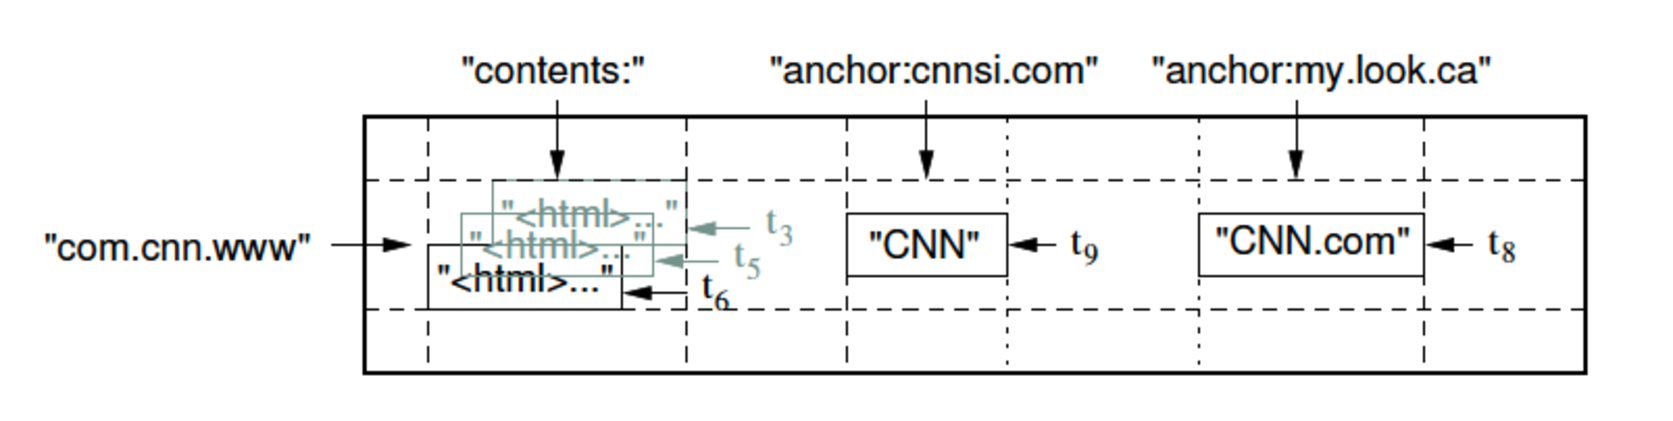
\includegraphics[width=5in]{../figures/bigtable.pdf}
\caption{HBase表结构(摘自\textit{Chang, F. et al. Bigtable: A distributed storage system for structured data. ACM Transactions on Computer Systems (TOCS), ACM, 2008})}
\label{fig:hbase}
\end{figure}

众所周知,在HBase中,数据是以表为单位存储的。表中的元素通过使用行关键字来区分,每一个行关键字都可以是任意一个字节串,而且HBase保证了所有针对字节串的读写都是原子的。如图\ref{fig:hbase}所示,HBase中的每一个表通常包含了数以亿行的数据,每一个行最多可以存储上千个列族以及上百万个列。列是以列族的方式组织起来的,每一个列族中可能包含不定数目的列,这些列可以在程序运行的过程中随时增加,列族也是进行访问控制的最小单元。每一个行列定位一个cell,其中存储着多个版本的数据。数据版本是一个64bit的整数。在cell中所有数据按照数据版本顺序以堆栈的方式堆叠起来。HBase中,如果想要使用某一个列族,开发人员必须事先新建该列族,或者通过改变表的属性来增加列族,列族被创建之后列才能被使用,用户通过指定’列族:列’来制定一个cell。前面提到了Domino是通过修改HBase来实现的,在Domino中,我们要求用户提交触发器的时候指定所要监控的事件,默认情况下就是数据更新事件。这个事件中必须制定所监测的表、列族,列则是可选的,如果不指定列,那么所有该列族中的列上的更改都会产生数据更新事件。


\begin{Sbox}
\begin{minipage}{5in}
\setlength\parindent{1pc}
\textbf{[分布式爬虫实例]}在Domino网络爬虫的实现中,我们需要监控两个数据写事件。一个来自由于爬取到新的微博数据而修改的WBContent表的列: ‘Content:zh’,另一个来自于由于猜测到某些用户可能最近更新了微博页面的WBUser表的列:’Activity:recently’. (触发器WBContentTrigger所监控的表如\ref{table:wbcontent}所示,而触发器WBUserTrigger所监控的表如\ref{table:wbuser}所示)。
\end{minipage}
\end{Sbox}
\shadowbox{\TheSbox}

\begin{table}[hb]
	\begin{minipage}[t]{0.5\linewidth}
	\centering
	\caption{\textit{WBContent} table in HBase}
	\label{table:wbcontent}
	\begin{tabular}{|c|c|c|}
		\hline
		\textit{MessageId} & \textit{Content:zh} & ...,... \\
		\hline
		\textit{Message-1} & $content_{1}$ & ...,... \\
		\hline
		\textit{Message-2} & $content_{2}$ & ...,... \\
		\hline
		... & ... & ...\\
		\hline
	\end{tabular}
	\end{minipage}
	\begin{minipage}[t]{0.5\linewidth}
	\caption{\textit{WBUser} table in HBase}
	\label{table:wbuser}
	\centering
		\begin{tabular}{|c|c|c|}
			\hline
			\textit{User Id} & \textit{Activity:recently} & ...,... \\
			\hline
			\textit{User-1} & $true$ & ...,... \\
			\hline
			\textit{User-2} & $true$ & ...,... \\
			\hline
			... & ... & ...,...\\
			\hline
		\end{tabular}
	\end{minipage}
\end{table}

\subsubsection{条件(Condition)}
条件是一组用户自定义的函数,该函数的传入参数是封装好的事件,返回值为true或false来表明当前用户制定的条件是否满足。在Domino中,条件(condition)包括了三种,分别负责三个关键的责任:首先,由于触发器一旦提交到系统中就会持久存在,除非用户显式的取消该触发器,然而在很多情况下,我们希望触发器能够在到达某些条件的时候自动停止,在这种情况下,用户就可以通过编写停止条件(stop condition)来实现判断。除此之外,由于Domino中的事件都是由数据写入引起的,如果短期内写入频率非常高,对它们进行快速处理就会极大的占据系统资源,在这种情况下,用户就可以通过编写间隔条件(interval condition)来为每一个触发器指定执行的周期。其实在Domino中,每一个活跃的触发器都是有一个最大执行频率的,用户可以通过编写条件函数覆盖该设置以加入自己的频率控制语句。最后,Domino还引入了选择条件(select condition)来对事件进行选择,仅仅处理其中一部分事件,该条件对于很多高效应用非常重要。

停止条件(stop condition)中非常的应用在那些迭代收敛的应用中。比如PageRank或者很多机器学习算法,这些算法中,往往需要判断连续两次迭代中计算的值之差是否足够小。如果足够小,程序就可以停止运行。Domino对这种应用做了特别的优化,每一个传入条件函数的封装好的事件都包括了更新前的值和更新后的值。

\begin{Sbox}
\begin{minipage}{5in}
\setlength\parindent{1pc}
\textbf{[分布式爬虫实例]}对于爬虫来说,我们不需要特别的停止语句,因此我们将默认使用Domino本身提供的条件函数(如\ref{code:wbcrawler}的filter函数所示)。
\end{minipage}
\end{Sbox}
\shadowbox{\TheSbox}

\subsubsection{动作(Action)}
动作函数(Action)是由用户编写的一段代码块来执行所需要的代码逻辑。Domino为用户的动作函数提供了完整的变量封装以提高用户代码执行的效率,如\ref{code:wbcrawler}中的HTriggerEvent对象。在该对象中,Domino为用户程序封装了多个相关值供其操作,这些值包括:触发该事件的数据更新动作相关的行关键字的值;该触发器所监测的列族或者列中数据的新值以及更新操作之前的旧值;事件发生的时间和上次同样的事件发生的时间。除此之外,我们还封装了相关的环境变量。比如触发器执行时所在节点的信息以及某些用户提交触发器时显式设置的变量及其值。

Domino为用户提供的是面向数据的编程模型,其允许用户在动作函数中任意访问需要的数据并且加以修改,并不需要像MapReduce或者Storm模型那样,必须按照流的概念来访问数据。这种方式简化了用户代码,不过也带来了问题。首当其冲的就是效率问题,允许用户在高频执行的动作函数对分布式存储系统(HBase)中的数据任意读写,特别是写,将给存储系统带来极大的压力,并且也会严重影响动作的执行速度。因此我们为这种情况专门提供了延迟写的异步语义,用户在动作函数中对分布式存储系统的写操作会被缓冲在本地的WritePrepared实例中,直到该动作函数退出前统一调用flush函数实施真正的写入操作。这一部分详细内容我们将在第\ref{section:io}部分进一步详述。

\begin{Sbox}
\begin{minipage}{5in}
\setlength\parindent{1pc}
\textbf{[分布式爬虫实例]}本应用中动作函数非常简单:对任意一条消息,找到所有曾经评论或者转发它的用户,并且将该用户的数据写入到WBUser表中。对每一个用户,爬取所有其最近发表的所有消息,并且存储到WBContent表中。具体的代码参见\ref{code:wbcrawler}中两个触发器中的action函数。
\end{minipage}
\end{Sbox}
\shadowbox{\TheSbox}

Domino模型在动作函数中一个关键的不同于现有的基于事件的分布式计算模型(比如Percolator或者Oolong)的地方:如何实现聚合操作。分布式爬虫的实例中不存在聚合操作,为了说明聚合操作的作用和重要性,我们这里简单的扩展该爬虫:当从某消息中获得所有曾经评论或者转发它的用户后,且将这些用户数据写入到WBUser表之前,出于某种原因,我们需要判断该用户所评论或转发的字数之和是否超过一定阈值,如果超过才认为他是活跃的并且写入到WBUser表以进行爬取工作。实现该功能,就需要搜集到所有同关键字的数据,并且加以聚合,就需要使用到聚合操作。

在Oolong这样的事件处理系统中,用户可以使用一系列显式的,事先定义好的聚合函数,比如求和、最大(小)值等。不过这些函数都太过简单,限制了实现很多复杂的逻辑的可能性。Google的Percolator完全没有对聚合操作提供额外的支持,所有的聚合动作都由用户通过使用事务机制自己实现(通常通过加分布式锁来实现),这对于不熟悉分布式系统的开发人员来说并不是一个好的选择。不同于已有系统,Domino设计了一个专用与聚合操作的设计模式:聚合模式。当用户需要聚合操作的时候,他可以完全按照聚合模式的指导来设计系统:首先,与原有触发器一起提交一个聚合触发器;其次,对所有需要聚合的触发器,修改其WritePrepared实例,引导结果写入到刚才提交的聚合触发器而不是HBase的表中;最后,通过修改聚合触发器中的动作函数来完成用户逻辑。通过这种方式,所有需要聚合的中间结果将被写入到一个隐式的表中($t_{acc}$),聚合触发器会自动检测该表上的变化,并且运行用户提交的动作函数。

引入聚合模式仅仅是解决了如何将来自不同的触发器动作产生的结果结合在一起的问题,紧接着的问题就是什么时候执行聚合模式中的动作函数:当来自不同服务器的触发器动作试图更新($t_{acc}$)中的数据时,它们往往是不同步的。然而,编程框架无法判断是否应该在触发器动作处进行同步等待或者可以异步向下执行,这跟应用程序有很大的相关性,因此Domino为不同的应用类型提供了不同的同步模型。

\subsubsection{代码节选}
\shadowbox{\textbf{[分布式爬虫实例]}}
\label{code:wbcrawler}
\begin{lstlisting}[language=java]
/**
 * WBContentTrigger.java
 */
package wbcrawler;

//所有提交的触发器都需要实现HTriggerAction这个基类
public class WBContentTrigger extends HTriggerAction{

  //访问微博的凭证
  private final String accessToken = @access_token;
  private WritePrepared writer = null;

  //初始化读写其他表中数据所用的WritePrepared实例。
  public WBContentTrigger(){
    byte[] tableName = "WBRelation".getBytes();
    this.writer = new WritePrepared(tableName);
  }

  private ArrayList<String> getUsersByAPI(String msgId);

  //封装好的事件对象,其中包括了触发事件的表、行以及相关列族的内容数据。
  @Override
  public void action(HTriggerEvent hte) {
    byte[] msgId = hte.getRowKey();
    byte[] msgContent = hte.getNewValue();
    String msgContentStr = new String(msgContent);

    ArrayList<String> aus = this.getUsersByAPI(new String(msgId));
    for (String userId : aus){
      Put p = new Put(userId.getBytes());
      p.add("Activity".getBytes(), "recently".getBytes(),
      		  "true".getBytes());
      this.writer.append(p);
    }
    this.writer.flush();
  }
  //过滤器,用来判断这个事件是否应该使触发器执行。
  @Override
  public boolean filter(HTriggerEvent hte) {
    return true;
  }
}
\end{lstlisting}
\begin{lstlisting}[language=java]
/**
 * WBUserTrigger.java
 */
package wbcrawler;
public class WBUserTrigger extends HTriggerAction{
  ...
  ...
  @Override
  public void action(HTriggerEvent hte) {
	byte[] userId = hte.getRowKey();
	Timeline tl = new Timeline();
	tl.client.setToken(this.accessToken);
	StatusWapper status = tl.getUserTimelineByUid(new String(userId));
	for (Status s:status.getStatuses()){
		Put p = new Put(msgId);
		p.add("Content".getBytes(), "zh".getBytes(), s.getText().getBytes());
		writer.append(p);
	}
	this.writer.flush();
  }
  @Override
  public boolean filter(HTriggerEvent hte) {
    return true;
  }
}
\end{lstlisting}

\subsection{同步模型}
\label{section:sync}
这里所说的同步和异步不同于I/O系统中的同步、异步模型。设想一下,在分布式程序中,如果当前计算需要分布运行的多个子任务产生的数据的时候,如何继续执行就是同步模型需要解决的问题。同步模型意味着计算的继续需要多有子任务的结果都已经产生;而异步模型意味着计算只需要发现有子任务产生了结果就可以继续运行。

\subsubsection{严格同步}

同步模型下运行的程序往往会带来很大的性能损失,这也很容易理解,因为程序的执行需要等待多个分布式子任务中最慢的那个完成才能继续,不过由于很多程序或者算法本身必须遵循该模型才能得到正确的结果,因此Domino中对该类应用提供了严格同步的原语以帮助实现这些算法。假设一个触发器在多个服务器上独立运行,并且在某一个节点需要一个严格同步的场景,在Domino中可以简单的通过使用同步模式来实现:在节点处实现一个聚合触发器,该触发器所配备的表会存储所有需要同步的中间计算结果。此时问题的关键就在于聚合触发器上的用户动作什么时候开始执行,它是如何知道所有需要同步的任务都已经执行到同步点了呢?

在Domino实现中,我们提供了两个原语($register$和$waitSync$)来提供严格同步的功能。首先所有需要进行同步的触发器动作刚开始执行的时候都需要先调用$register$来注册自己,每次注册成功后会在ZooKeeper中生成一个临时节点,节点的名字为triggger的id加当前执行序列id,该节点中存储一个count值,每次注册的时候将count值加1;当触发器动作执行完退出的时候会将ZooKeeper中对应的节点中的值减1,如果减一后节点值为0,那么就删除该节点。所有调用$waitSync$的动作函数都根据当前执行序列id,挂在ZooKeeper的对应节点上同步等待。当节点被删除的时候,$waitSync$返回,开始执行用户逻辑。此时可以保证所有需要同步的节点上的触发器动作都已经执行完毕了。


\subsubsection{完全异步}

与同步模型相比,异步模型是另外一个极端,它永远以分布式子任务中最快的那个为标准执行。相比之下明显具备更好的效率,并且很多算法都被证明异步结果和同步结果非常接近,并不会影响到结果的正确性。比如很多线性的数据挖掘和机器学习算法(belief propagation, expectation maximization, stochastic optimization, and PageRank etc)。Domino本身的触发器语义天然的支持了这种全异步的模型:触发器被自动的指派到不同的节点上独立执行。

\subsubsection{最终同步}

为了平衡很多同步应用对性能的要求,Domino除了提供同步异步模型外,还设计了一套最终同步的模型,专门用来提高那些需要较好的响应时间,且不能够简单改写为异步模型应用的性能。

\begin{figure*}[]
\centering
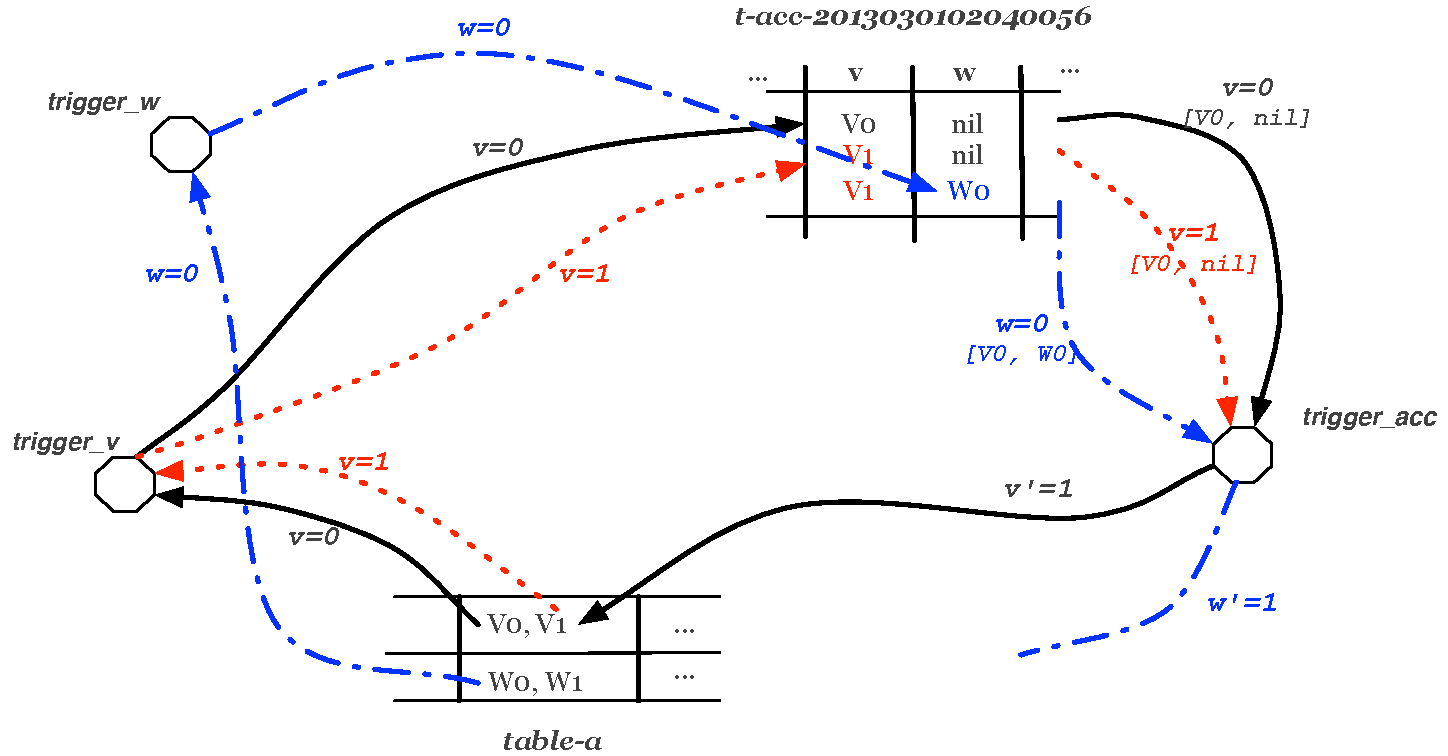
\includegraphics[width=5.5in]{../figures/multiv.pdf}
\caption{Domino中最终同步模型下多版本执行的流程图}
\label{fig:multiv}
\end{figure*}

最终同步模型中,程序的执行不需要等待所有的子任务都完成,程序可以提前向下执行,但是在足够的时间窗口后,最终还是会得到同步执行相同的结果。它不同于异步模型的地方在于,当前执行的程序的所有来自之前子任务的中间数据的版本号都必须满足一定的要求,以保证最终结果的正确性。因此,该模型下运行的应用能够具有较好的性能,并且有可能提前给出正确的结果。

Domino中最终同步模型基于HBase的多版本表实现,它可以用于同步两个不同的触发器,也可以用于上一节我们描述的聚合模式。比如,当用户需要聚合操作,并且需要在聚合操作处进行同步的时候,只要伴随需要聚合的触发器再提交一个聚合触发器即可。系统会自动创建一个仅本应用可以访问的隐式表,该表存储的所有数据都是带有版本信息的。表中任一个cell上数据的版本信息等于将该数据写入表的触发器动作的执行序列id,而触发器动作的执行序列id则是从0开始,每次执行自动加1的。聚合触发器的动作(Action)则根据表上的数据更新操作来执行:每次数据更新都会触发动作执行用户定义的聚合操作,那么这个动作的执行序列id就是更新后的数据的版本号。执行聚合操作需要读入表的数据,Domino模型确保该函数只能读到小于或等于当前执行序列id的数据,最终产生的结果的版本id也是当前动作的执行序列id加1。

图\ref{fig:multiv}展示了这样一个最终同步模型下多版本执行的流程。我们使用了两个触发器:$trigger_{[w|k]}$和$trigger_{acc}$来做示例。其中$triger_{[w|k]}$由表$table_a$触发,而$trigger_{acc}$用来帮助同步所有$trigger_{[w|k]}$实例产生的中间结果。表名字为t-acc-2013030102040056,由Domino系统自动创建,且仅在$trigger_{acc}$中可以访问。由图中可以看出$trigger_w$比$trigger_v$慢一些,当$v$已经运行到执行序列为1的时候,$w$刚刚开始它第0轮运行。那么在整个执行过程中,两个中间结果会被聚合触发器的动作函数根据输入$[v_0, nil], [v_1, nil]$计算出来并且写入到HBase的表中。这些结果未必正确,但是它能够作为中间结果被访问和使用。如果我们的算法中这些部分结果是有意义的,那么这些部分结果就能够被最早的加以利用,而不是所有的节点都等待最慢节点的执行。当然,随着$w$的执行,其最终也会将结果写入到表中,聚合函数根据版本顺序,取到的输入正好是所有同版本的数据,从而得到正确的结果。

最终同步相比较严格同步来说,不会发生停止等待的情况,不需要分布式锁的参与。特别对于那些中间结果有意义的算法具有非常好的效果,且其本身也可以保证最终结果与同步模型结果完全相同。因此在实际应用中有很多优势。不过其问题也非常明显,其中最大的就是资源浪费问题,如果大量的中间结果是无意义的,那么浪费计算资源去计算它们就没有意义。因此对于这类算法,还是应当采用严格同步的模型。

由于在最终同步的实现中,所有的序列id都是本地维护的,这样就存在一种可能性:具有相同执行序列的动作函数都试图向同一个位置发起写操作。在这种情况下,我们需要对这些写操作指定一个顺序来保证结果的正确性。在Domino中,我们定义一个触发器的某个动作函数的写序向量如下:
\begin{equation}
V^{T} = (V_{tc_{fired}}: V_{tc_1} : V_{tc_2}: ... V_{tc_i})
\end{equation}
其中等式右边的$V_{tc_{fired}}$代表触发该触发器动作执行的数据版本号,而$V_{tc_i}$则代表了触发器动作执行时访问的数据的版本号。当两个具有相同的触发器动作执行序列号的动作($i$和$j$)试图向同一个位置写入数据的时候,系统将比较他们的写序向量:首先比较$V_{tc_{fired}}^i$ 和 $V_{tc_{fired}}^j$,较大的动作写入;若相等,那么从前向后依次比较$V_{tc_i}$,同样是较大的动作写入。

通过这种方式设计的写顺序,通过简单的分析就可以知道:任何时候,一个全部到达同步点的写入带来的触发器动作一定比所有未完全到达同步点的触发器动作的写序向量大,这样就保证了最终同步的结果不会被覆盖。

\section{设计和实现}
\label{section:design}
本节中我们将介绍Domino运行时系统的实现以及其重要挑战的解决方法。首先图\ref{fig:arch}展示了Domino不同模块之间的逻辑架构。

\begin{figure}[ht]
\centering
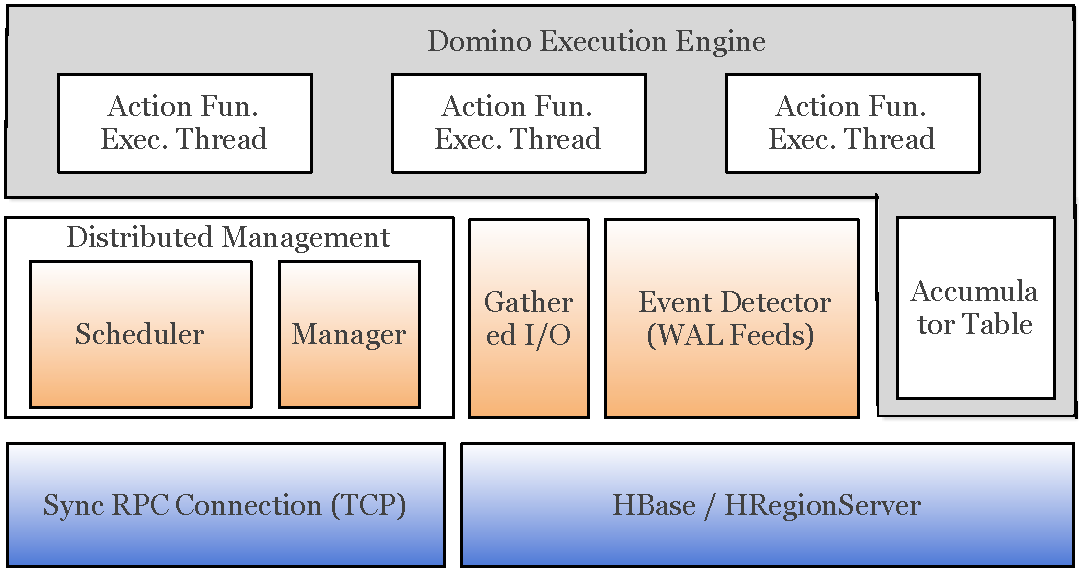
\includegraphics[width=5in]{../figures/arch.pdf}
\caption{Domino运行时系统的模块图,每一个模块都依赖于其下面模块提供的服务}
\label{fig:arch}
\end{figure}

Domino本身是基于HBase实现的,因此在实际运行中其节点之间的架构和HBase一致,都是由Master节点和Slave节点组成。HBase中的Master节点称为$HMaster$,slave节点也就是实际的Region存储的节点被称为$HRegionServer$;于此对应的是Domino的节点,Domino的Master节点$TriggerMaster$与HBase的$HMaster$运行在同一个物理节点上,而任务执行节点$TriggerWorker$运行在$HRegionServer$的节点上。所有的节点都运行着图\ref{fig:arch}中的各个组件,唯一的区别是$TriggerMaster$会运行其中的分布式管理(distribted management)部分,而$TriggerWorker$则不会运行这部分。不同的$TriggerWorker$之间通过同步的RCP远程调用来互相通信,而所有的$TriggerWorker$也需要和$TriggerMaster$保持一个心跳连接以汇报所有触发器的执行状态。需要注意的是,Domino的$HMaster$不是由用户手工指定的,而是在Domino启动的时候首次将自己注册成为$TriggerMaster$的节点充当。因此在Domino中不存在单点故障或者单点性能瓶颈。

\subsection{执行流程}
用户想Domino系统提交触发器采用MapReduce任务提交类似的方式:首先将需要执行的触发器相关代码打包成jar包,然后通过domino命令行程序提交到系统中去。下面的代码块展示了如何将上文中实现的分布式触发器提交给Domino的命令。其中WBCrawler为一个包含了main入口的主类,其负责提交另外WBContentTrigger和WBUserTrigger。
\begin{lstlisting}[language=bash]
	bin/domino trigger WBCrawler.jar wbcrawler.WBCrawler
\end{lstlisting}

用户向Domino提交触发器是通过新建并初始化一个Trigger对象,之后调用其submit方法实现的。下面的代码块展示了分布式爬虫实现中一个触发器(WBUserTrigger)的提交代码。用户需要新建一个Trigger对象,这个对象中必须设置触发器的名字,指定所监测的表、列族信息。如果这个触发器的检测对象具体到列族中的某个列,那么还需要调用配套的设置函数来设置,最后最重要的是需要设置该触发器触发时执行的类。这个类中应当包括用户实现的条件函数和动作函数。

\begin{lstlisting}[language=java]
Trigger tg2 = new Trigger("WBUserTrigger", "WBUser", "Activity");
tg2.setTriggerOnColumn("recently");
tg2.setActionClassName("wbcrawler.WBUserTrigger");
tg2.submit();
\end{lstlisting}

调用Trigger对象的submit函数后,Domino会首先从$TriggerMaster$处获得一个全局唯一的触发器id,之后将用户提交的jar包提交到HDFS存储系统由该触发器id组成的目录中。之后所有的$TriggerWorker$都将HDFS的该位置下载并加载需要的类。Domino会首先向$TriggerMaster$提交触发器。提交成功之后,会询问HBase的.META.表来获取本触发器所监测的表所在的$RegionServer$的位置。之后会依次向这些$RegionServer$提交触发器请求。只有所有的触发器请求都成功之后,提交才会返回。如果其中出错,Domino会负责回滚之前的操作,并且返回用户提交失败的信息。

触发器提交成功之后就已经开始在$RegionServer$处开始运行。此后,Domino在每一台服务器上都运行着事件感知组件(\ref{subsection:feed})负责监控数据更改,当遇到对象的数据修改的时候,用户提交的触发器代码就会被加载执行。触发器会因为停止条件(stop condition)而停止,也可以由用户提交命令显示的停止。在Domino中,用户程序可以使用Trigger对象的stop()方法来卸载一个触发器,也可以使用shell命令来完成:
\begin{lstlisting}[language=bash]
	bin/domino stop_trigger trigger-id
\end{lstlisting}
命令提交后,Domino会首先根据用户提交的‘trigger-id’来查找对应的trigger实例。如果存在,就会先卸载运行在$TriggerWorker$上的实例,所有实例卸载完成之后再卸载$TriggerMaster$上的实例,完成后返回。

\subsection{事件感知组件}
\label{subsection:feed}
Domino的事件感知组件包括两部分。第一部分(WAL Feeds)作为主要的事件感知源用于在正常情况下对数据修改进行快速的感知;而另外一部分(Sequential Scan)则作为持久化事件的组件存在,当系统中出现错误的时候,该部分则保证所有未处理的事件都不会丢失。

\subsubsection{WAL Feeds}

HBase是一个保证了数据持久存储的分布式存储系统,它不会因为少量节点的故障而丢失数据。这是因为其会将所有的数据都存储在磁盘中,而磁盘则利用HDFS提供的多备份来保证数据的安全性。然而由于磁盘的响应时间过慢,为了提高IO性能,HBase会将所有的数据暂时存储在内存中,同时持久化在HDFS的WAL(write-ahead-log)中。为了保证数据不会因为在写操作的过程中节点突然崩溃而丢失,HBase会先将数据写入到WAL中,并且在写入成功后才开始将数据写入到内存中。写入到WAL中的数据是按照其在内存中的结构组织来写,而是将每一条数据整理成包括:行关键字、列族、列、值、时间戳、类型的日志,以顺序的方式写入WAL文件中,以提高磁盘I/O性能。

Domino的事件感知组件利用了HBase存储数据的特点,在每一个$TriggerWorker$中,Domino的事件感知组件都会将自己注册到HBase写入WAL文件的关键路径中,完全异步地对当前写入的日志数据进行判断,判断是否属于某个已注册的触发器所监测的范围。

\begin{figure}[]
\centering
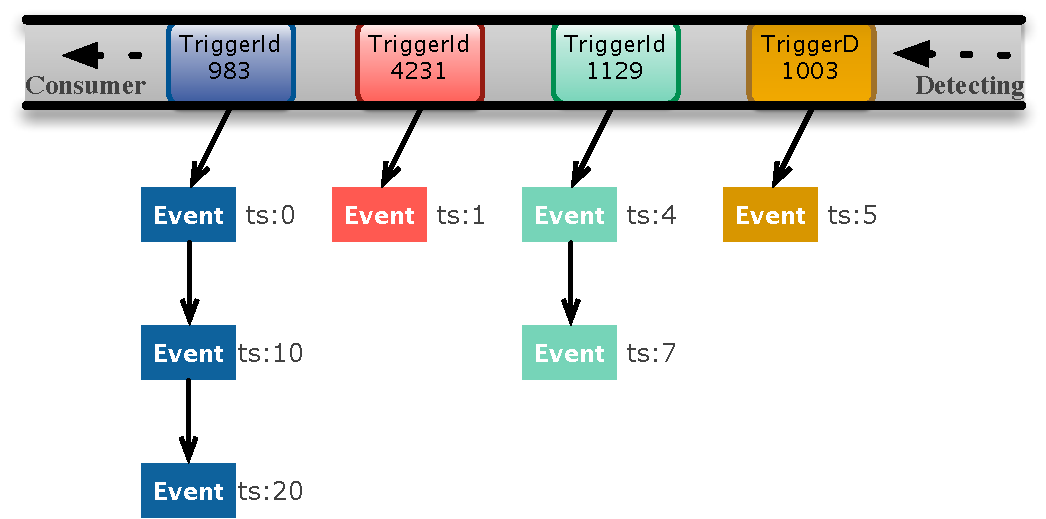
\includegraphics[width=5in]{../figures/queue.pdf}
\caption{Domino事件队列。如果两个事件属于同一个触发器,它们会整合被放入到队列中的同一个位置。队列中的顺序基于时间戳。消费者每次队列中取出属于同一个触发器的所有事件以减少频繁的进行线程切换带来的性能损失。}
\label{figs:queue}
\end{figure}

一旦事件感知组件探测到了一个对WAL文件的修改,并且该修改正好属于某一个已经注册的触发器的监测范围,它将封装一个包括了更新后的值以及更新前的值的事件(HTriggerEvent)并且将封装好的事件对象放入到事件队列中(如图\ref{figs:queue})所示。队列上有一个消费者不断的从队列中取出最新的事件来处理。最终,触发的事件会被发送到用户所写的条件函数和动作函数来处理。为了进一步提高效率,我们在每一个$TriggerWorker$中预先开辟了一个线程池,且为每一个触发器启动了一个线程,并且空置等待着事件到来执行。在实际的实现中,我们扩展了Java的同步线程库,使得所有的线程都变得可管理。具体表现在所有的子线程都有自动的异常处理、执行状态记录、重启等功能。

\subsubsection{Sequential Scan}
WAL Feeds 组件对事件相应时间较低,适合作为主要的事件感知组件在Domino中运行。然而由于它的核心组件——事件队列是一直存在与单节点的内存中的,如果节点出现故障就无法恢复。这对于一个会长时间运行的分布式运行时系统来说是不可以接受的。为了在保证事件感知效率的前提下提高系统容错的能力,我们引入了Sequential Scan的策略来为Domino提供错误情况下的事件探测工作。

首先,由于Domino允许最小的监测单元是列,而HBase本身是将表按照列族分为独立的单元来管理的,因此同一行且同一个列族的数据一定在同一台服务器上存储着。我们修改HBase代码,为每一个列族默认的增加一列(\_events\_),每次HBase在向某一列族中的某一列写入数据的时候,系统会同时在\_events\_列中存储此次写入的本地唯一id,这个本地唯一id也会被存储到$HTriggerEvent$对象中,传给动作函数。用这样的方式,在WAL文件中,就会生成连续的两条写入日志:数据列写入和\_events\_列写入。另外一方面,当用户提交的触发器动作函数执行完毕的时候,Domino会自动将id从\_events\_列中删除。

如果Domino在运行过程中,某个节点崩溃,那么我们在WAL Feeds中所构造的事
件队列全部丢失,此时触发器会在另外一个节点上重新启动,而所有的崩溃节点
的数据也会在另外一个节点上由WAL文件进行恢复。在恢复的过程中,我们可以首先获得每一行数据,每一个列族的\_event\_列最新数据。上面记录了在事件队列中丢失了的所有的写入时的id。对每一个id,从后向前,逆着事件顺序搜索,当发现带有该id的WAL日志的时候,其前面那一条日志中存储的数据就是导致事件发生的,更新的数据的值。Domino会强制重新产生这个事件,进而继续之前未能执行的触发器动作。


\subsection{延迟写组件}
Domino为用户提供了面向数据的编程模型,它允许用户在自己编写的函数中自由的访问数据。但是这种模型也会带来很多问题。首当其冲的就是性能问题,因为访问非本地数据是非常耗时的,而用户写的函数中可能多次调用这样的写操作从而使得情况更加糟糕。另外一个问题就是数据的一致性问题,前面在介绍最终同步的时候,我们介绍了如何解决同一个触发器不同的动作之间写冲突时一致性的方案,而这里需要考虑的是不同触发器的写冲突。首先,对于单个写操作,在Domino中,我们始终保证后写成功。在这个前提下,我们面临一个更复杂的情况:由于我们允许用户自由的读写数据,那么有可能发生不同的触发器动作会进行交错的写操作。比如触发器A写入$loc_1$,且成功,之后开始写$loc_2$;而触发器B先写入$loc_2$成功后写入$loc_1$,这样最后结果是$loc_1$被A写入,$loc_2$被B写入,任何一个触发器内部都无法得到一个一致的状态。

为了解决这些问题,在Domino中,我们提供了一个延迟写组件(WritePrepared)帮助提高写效率,同时帮助在一个触发器内部维持一个一致的数据状态。WritePrepared封装所有在触发器动作函数中发起的对HBase表格的写操作,并且通过在一次动作函数执行完毕的时候调用flush方法来一次性的将WritePrepared中缓存的数据真正写入到HBase的表格中。

WritePrepared中的缓存数据写入HBase表时是有序的,顺序是由调用flush操作的时候从ZooKeeper获得的全局序列id($G_{id}$)决定的。当两个具有不同全局id的写操作从Domino的触发器中发出的时候,如果两者并没有冲突(即没有写入同一个位置),那么HBase并不会感受到有什么不同;然而如果两者产生冲突,那么具有较大的全局序列id的写操作会被挂起直到前一个写操作完成。在挂起期间,所有之前部分写成功的数据都会被冲突的那个、具有较小的全局序列id的写操作覆盖。WritePrepared的flush顺序并不意味着我们将所有的分布式写操作都强制排序了。强制对所有写操作排序会极大的降低写性能,我们只是通过版本控制保证具有较低的全局id的flush操作开始后,它就不会被别的触发器抢占。

使用WritePrepared和flush操作,我们可以为触发器中的动作函数提供较高的I/O效率,并且保证所有的写操作不会互相交错。

\subsection{容错和恢复组件}
容错能力是云计算平台下的计算模型面临的的最大的挑战。很多流式计算模型,像Storm和S4这样的系统虽然具有较好的性能,但是其在容错和恢复上的短板同样极大的限制了其应用。然而,Domino由于采用了基于触发器的模型,所有的中间数据都可以保存在持久存储的分布式存储环境中使得我们能够有机会提供一个让人印象深刻的容错能力以及一个近乎实时的错误恢复能力。

首先,Domino的各个组件通过HBase提供的容错能力作为其静态容错的基础:所有提交的触发器信息都存储在HBase中,所有中间数据都被保存在HBase表中,触发器的执行状态也通过序列id区别保存,甚至聚合模式中自动创建的分布式表($t_{acc}$)也持久存储在HBase中。这些信息都不会因为节点的意外崩溃而丢失。

除了静态容错外,由于触发器在Domino系统中时刻处于运行的状态,我们希望能够对执行中的状态实现容错和恢复。比如正在执行的触发器所在的节点崩溃,或者触发器本身线程崩溃,我们希望能够尽快的在备份节点上继续之前正在进行的计算。

Domino节点中比较极端的情况是物理节点崩溃,这也意味着其上面运行的HBase服务也离线。那么节点崩溃之后的所有更新操作都会被重定向到自动选出的备份节点,并且在备份节点上会开始根据WAL中的数据重建内存数据结构。在备份节点恢复数据的同时,Domino的触发器会随之重新在备份节点上初始化并且开始运行。这意味着,所有在节点崩溃之后新的数据写入操作都会如同没有发生错误一样在新的节点上被触发器监测并且处理。而对于那些崩溃发生时正在执行的动作函数来说,所有能影响到HBase的输出都被缓存在WritePrepared中。若崩溃时尚未执行到flush,那么该动作函数的本次执行未完成,Domino在备份节点上重新运行该动作函数即可(只读入对应该执行序列id的输入数据);若崩溃时已经开始执行flush,那么这次动作函数的执行其实已经完成,只剩下最后的IO操作。为了能够保证完成所有的缓存在WritePrepared中的IO操作,在Domino中,除了前面所讲每一个的WritePrepared都在ZooKeeper中申请全局唯一序列号($G_{id}$)外,我们还为每一个WritePrepared实例都在ZooKeeper上映射了一个临时节点,其中存放序列化好的HBase写入操作序列以及当前执行完的操作id,这样保证一旦flush开始就一定能够完整结束。

\subsection{异常控制}
The action functions submitted by programmers in Domino are different from MapReduce jobs as Domino’s action func- tions are executed in the same JVM where HBase compo- nents are running at, however the new MapReduce jobs are running at new JVMs. The reason we can not start stan- dalone JVM for each action function is there may be hun- dreds of active triggers waiting on one server instead of lim- ited job slots in MapReduce. If we start each trigger a JVM, it will soon consume all the resources. So, we start a thread pool to execute each trigger inside the HBase’s JVM.
In fact, it is dangerous to run users’ programs inside HBase’s JVM, so we provide thread manager for all threads which will be attached by trigger action functions. We catch every Throwable objects (which is the very basic class for all the errors and exceptions in Java) for the standalone thread and restart these threads according to their recorded status.

\subsection{优化}
As we have described before, Domino provides develop- ers some unique features which would be greatly helpful to write large scale applications. However, the disk-based stor- age systems (HBase) and the trigger-based model still in- troduce some performance penalty. For example, during the execution of any trigger, we need to write all the interme- diate values into tables in HBase to trigger another trigger even if, in many cases, we do not care about the interme- diate results. So, to accelerate the performance of Domino applications without wasting the valuable system resources, we introduce a serial of optimizations. And we will describe some significants of them in this section.
\subsubsection{内存加速}
To provide persistency guarantee, HBase will write all up- dates into WAL(write-ahead-log) before writing into local memory structure. And, in section 4.1, we introduced how Domino uses this WAL files to detect the cell updates in HBase tables. However, As we have mentioned, not all the intermediate results are necessary to be stored into HBase table persistently because we only care about the final results and writing into WAL files consumes much more time than writing into local memory due to high disk I/O latency.

To speedup the execution of Domino applications, we in- troduce in-memory shadow table, which is created automat- ically by Domino system. The shadow table will always be created as a shadow of an existing HBase table, which the trigger is monitoring on. In case that developers turn on the shadow table option, the shadow table will be created once the trigger is submitted successfully. Inside the trigger execution, all the writes in Domino system will firstly be directed into the shadow table before into the real HBase ta- ble. Each shadow table is only visible inside the trigger who creates it, so when data was written into the shadow table, the relevant trigger will detect the event through monitoring on the in-memory shadow table instead of HBase table, and other triggers are still motivated by HBase table or their own shadow tables. As the shadow table is stored in memory and does not need to provide persistency guarantee, it can provide a much better performance.

Using shadow table leverage the performance a lot in Domino system: in some cases, it can provide 2-3X speedup compar- ing with original Domino. However, developers should be aware of using this feature in a long time running applica- tion because the failures of these in-memory shadow tables will cause the whole application re-run. If we want to run the applications really fast, we should divide the long time applications into several small triggers to reduce the possi- bility of re-run the whole programs.

\subsubsection{负载均衡}
Applications running in Domino always keep locality be- cause all the actions are executed right on the server where the event is fired. If part of a table is facing more updates than others, then the server where this part was stored will run more actions. We call this part of table the hot spot. To balance the loads across different servers, we need distribute these hot spot into different servers. In HBase, each region represents a continuos part of a table, and these regions will be auto splited into two daughter regions and possibly be dis- tributed into two different servers when they grows larger. In Domino, we issue the splitting signals when we found some regions are hot spot even they are not large enough. After splitting it into two sub-regions, we will distributed one of them into a low load server to make the Domino cluster load balance. Whenever the regions are moved to other nodes, the triggers that monitor on them will also copied or moved to other nodes. All these trigger-node-region mapping information is stored in the TriggerMaster node.

\subsubsection{与别的框架一起工作}
Domino was designed to be a general programming frame- work for applications running in Cloud environment, but it still has its advantages and disadvantages. For example, some algorithms only contain simple round-by-round math- ematic computations and each round computation needs global information that generated in last round. Implementation this kind of algorithm in Domino needs some tricks (like k-means in next section), which is not necessary if using some extended MapReduce frameworks like Spark, which will provide very convince performance and conciseness.
However, in such problems, Domino still should work as a necessary component to provide the critical incremental ability for applications. Developers do not need to change their MapReduce codes or their Domino codes, these different frameworks can work together to provide a good optimization. The combination between Domino and other frameworks includes two steps. Firstly, an offline MapReduce application calculates the initial results from large amount of input dataset. Then, the Domino applications which monitors on the input dataset will run and generate continuos correct results during new input dataset is coming.

\section{应用实例}
\label{section:apps}
As we have introduced in the beginning of this paper: Domino was designed as a general programming framework in Cloud. To demonstrate this, we have implemented several more applications: a distributed web crawler for social network, collaborative filtering[34] for movie recommendation, k-means parallel computation. In this section, we will firstly summarize how Domino’s programming model enables efficient implementation for these applications and then introduce the performance advantages brought by Domino in next section.
\subsection{PageRank算法}

\subsection{协同过滤算法}
\subsection{$K$-means算法}

\section{实验分析}
\label{section:exp}
\subsection{HBase性能比较}
\subsection{扩展性分析}
\subsection{与MapReduce比较}

\message{ !name(chap-domino.tex) !offset(-367) }
